\subsection{Record Dialogue GUI Change}
By satisfiability testing it was found that the Record Dialogue should be changed again.

\begin{figure}[h]
        \centering
        \begin{subfigure}[b]{0.3\textwidth}
                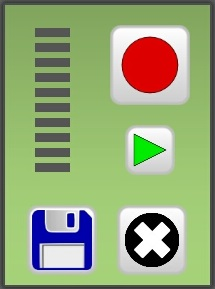
\includegraphics[width=\textwidth]{sprint2/recorddianoaction}
                \caption{Idle mode}
                \label{fig:recordnoaction}
        \end{subfigure}%
        ~ %add desired spacing between images, e. g. ~, \quad, \qquad etc.
          %(or a blank line to force the subfigure onto a new line)
        \begin{subfigure}[b]{0.3\textwidth}
                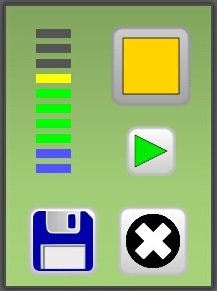
\includegraphics[width=\textwidth]{sprint2/recorddiarecording}
                \caption{Recording mode}
                \label{fig:recordrecording}
        \end{subfigure}
        ~ %add desired spacing between images, e. g. ~, \quad, \qquad etc.
          %(or a blank line to force the subfigure onto a new line)
        \begin{subfigure}[b]{0.3\textwidth}
                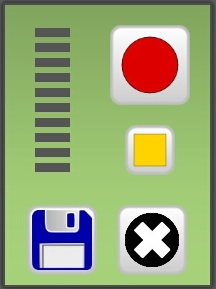
\includegraphics[width=\textwidth]{sprint2/recorddiaplaying}
                \caption{Playing mode}
                \label{fig:recordplaying}
        \end{subfigure}
        \caption{Record Dialogue GUI}\label{fig:recorddia}
\end{figure}

The record dialogue GUI to be changed was the one seen in \figref{fig:record-dialogue}.
However, the customers desired fewer buttons, and pointed out that the play and stop button could be combined into one button, as they are mutual exclusive.

To support this change, the audio player was changed to the Android \textit{MediaPlayer} instead of \textit{SoundPool}, as \textit{MediaPlayer} supports an event for registering when a sound is finished playing.
The new GUI can be seen in \figref{fig:recorddia}.
It was shown to the customers and they found it reflected their requirements.